%%%%%%%%%%%%%%%%%%%%%%%%%%%%%%%%%%%%%%%%%%%%%%%%%%%%%%%%%%%%%%%%%%
%%%%%%%% ICML 2013 EXAMPLE LATEX SUBMISSION FILE %%%%%%%%%%%%%%%%%
%%%%%%%%%%%%%%%%%%%%%%%%%%%%%%%%%%%%%%%%%%%%%%%%%%%%%%%%%%%%%%%%%%

% Use the following line _only_ if you're still using LaTeX 2.09.
%\documentstyle[icml2013,epsf,natbib]{article}
% If you rely on Latex2e packages, like most moden people use this:
\documentclass{article}

% For figures
\usepackage{graphicx} % more modern
%\usepackage{epsfig} % less modern
% \usepackage{subfigure}
\usepackage{subcaption}
\usepackage{multicol}

% For citations
\usepackage{natbib}

% For algorithms
\usepackage{algorithm}
\usepackage{algorithmic}

% For math
\usepackage{amsmath}
\usepackage{siunitx}

% As of 2011, we use the hyperref package to produce hyperlinks in the
% resulting PDF.  If this breaks your system, please commend out the
% following usepackage line and replace \usepackage{icml2013} with
% \usepackage[nohyperref]{icml2013} above.
\usepackage{hyperref}

% Packages hyperref and algorithmic misbehave sometimes.  We can fix
% this with the following command.
\newcommand{\theHalgorithm}{\arabic{algorithm}}

% Employ the following version of the ``usepackage'' statement for
% submitting the draft version of the paper for review.  This will set
% the note in the first column to ``Under review.  Do not distribute.''
\usepackage{icml2013}
% Employ this version of the ``usepackage'' statement after the paper has
% been accepted, when creating the final version.  This will set the
% note in the first column to ``Proceedings of the...''
% \usepackage[accepted]{icml2013}


% The \icmltitle you define below is probably too long as a header.
% Therefore, a short form for the running title is supplied here:
\icmltitlerunning{6.867: Homework 2}

\begin{document}

\twocolumn[
  \icmltitle{6.867: Homework 2}

  % % It is OKAY to include author information, even for blind
  % % submissions: the style file will automatically remove it for you
  % % unless you've provided the [accepted] option to the icml2013
  % % package.
  % \icmlauthor{Your Name}{email@yourdomain.edu}
  % \icmladdress{Your Fantastic Institute,
  %             314159 Pi St., Palo Alto, CA 94306 USA}
  % \icmlauthor{Your CoAuthor's Name}{email@coauthordomain.edu}
  % \icmladdress{Their Fantastic Institute,
  %             27182 Exp St., Toronto, ON M6H 2T1 CANADA}

  % You may provide any keywords that you
  % find helpful for describing your paper; these are used to populate
  % the "keywords" metadata in the PDF but will not be shown in the document
  \icmlkeywords{boring formatting information, machine learning, ICML}

  \vskip 0.3in
]

\section{Logistic regression}
In this section, we explore logistic regression with L1 and L2 regularization. We use gradient descent to compare the resulting weight vectors under different regularizers and regularization parameters, and we evaluate the effect of these choices in the context of multiple data sets.

\subsection{L2 regularization}
We first consider L2 regularization, in which the objective function to minimize is
$$E_{LR}(w, w_0) = \textsc{NLL}(w, w_0) + \lambda ||w||^2_2$$
where
$$\textsc{NLL}(w, w_0) = \sum_i \log(1 + \exp(-y^{(i)} (w x^{(i)} + w_0)))$$
and in the case of L2 regularization,
$$||w|| = |w|_2 = \sqrt{w_1^2 + ... + w_n^2}$$
Gradient descent was run with this objective function on the training dataset \texttt{data1\_train.csv} with $\lambda = 0$. We observed how the weight vector changed as a function of the number of iterations of gradient descent across various initial guesses, step sizes, and convergence criterion. There were three key findings that we were able to make. First, we saw that the ultimate convergence weight was heavily dependent on the initial guess. This actually makes a good deal of sense because of the fact that there are infinitely many ways to perfectly separate a dataset that's linearly separable. The second observation was that $w_{0}$ and $w_{1}$ always decreased as number of iterations increased whereas $w_{2}$ also increased. Finally, we saw that the convergence weight values were all within the same order of magnitude as the initial guess. This makes intuitive sense since we know from class that in the case of linearly separable data, the optimization aims to make the weights as large as possible.

When $\lambda = 1$, we see drastically different behavior in how the weight vector changes throughout the course of the gradient descent. The primary difference is the fact that $w_{0}, w_{1},$ and $w_{2}$ all converge to much smaller values. For example, when we set the initial guesses to be $100$ for all 3 components of the weight vector, the converged weights were two orders of magnitude less than the initial guesses. The reason for this phenomenon is due to the regularization penalty incurred when we set $\lambda = 1$

\subsection{L1 regularization}
In the case of L1 regularization, the objective function is the same except that $||w^2_2||$ becomes replaced with $||w_1||$, whereby $||w_1||$ is defined by:
$$|w| = |w|_1 = \sum_{i=1}^n |w_i|$$
We can evaluate the different regularization techniques under different values of $\lambda$ in the context of the weight vectors, the decision boundary, and the classification error rate in each of the training data sets. Before we dive into details, we make the obvious observation that when $\lambda = 0$, the choice of regularizer ($L_1$ vs. $L_2$) makes no difference on anything since the entire term is just $0$.

\subsubsection{Weight vector}
In terms of the weight vector, we discovered that depending on whether the particular $|w_n|$ was less than or greater than $1$ either the L1 regularization resulted in a higher magnitude weight or the L2 regularization resulted in a higher magnitude weight. Specifically, when $w_n$ was less than 1, L2 regularization resulted in a higher magnitude weight, whereas when $w_n$ was greater than 1, L1 regularization resulted in a higher magnitude weight.   This makes intuitive sense because squaring number larger than 1 results in larger numbers while squaring numbers less than 1 result in smaller numbers. We also discovered that a larger $\lambda$ values resulted in smaller weight magnitudes for both L1 and L2.

\subsubsection{Decision boundary}
The decision boundary was able to perfectly separate the data for all values of $\lambda$ as well as for both L1 and L2 regularization when the dataset was linearly separable. Generally, all the decision boundaries looked very similar to one another across values of $\lambda$ as well as for both L1 and L2 regularization. The one slight difference we noticed is that when $\lambda = 0$ the algorithm tried to correctly classify the greatest number of points without maximizing margins, whereas when $\lambda=1$ the algorithm was able to divide the data into more evenly spaced clusters. This makes sense because $\lambda$ is the regularization parameter on the weights, so when $\lambda = 0$, the weights can increase without penalization to fully account for the data. When $\lambda = 1$, however, higher magnitude weights were penalized, thus resulting in division of the clusters more evenly.

\subsubsection{Classification error rate}
The classification error rate was always $0$ for all values of $\lambda$ as well as for both L1 and L2 regularization when the dataset was linearly separable. For datasets that were not linearly separable, we found that a larger $\lambda$ generally resulted in slightly worse performance for the training sets (for example, 0.9875 with $\lambda = 0$ and 0.965 with $\lambda = 1$ for training dataset 2 using L1 regularization.

\subsection{Optimization}
By using the training and validation data sets, we can identify the best regularizer and value for $\lambda$ for each of the four data sets. These results are presented in Table 1 (above). Graphs of the decision boundaries for the optimal regularizers and $\lambda$s are shown below.

\begin{table}
  \begin{center}
    \begin{tabular}{ | c | c | c | c | }
      \hline
      Data & Best regularizer & Best $\lambda$ & Test performance \\ \hline
      1       & both           & all            & 1.0 \\ \hline
      2       & both           & all            & 0.805 \\ \hline
      3       & L2               & 1             & 0.97 \\ \hline
      4       & L1               & 1             & 0.5 \\ \hline
    \end{tabular}
  \end{center}
  \caption{Optimal regularizer and $\lambda$ for datasets}
\end{table}

\begin{figure}[width=\linewidth]
\centering
\begin{multicols}{2}
  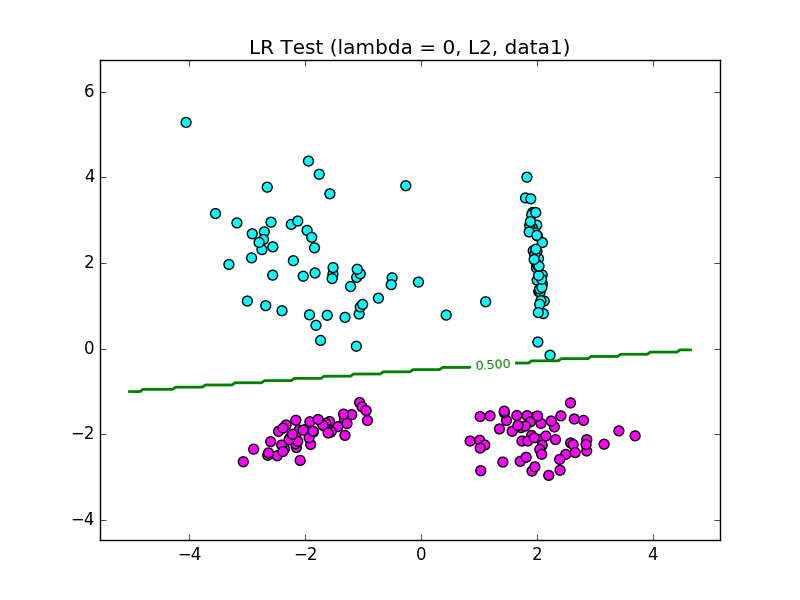
\includegraphics[width=1.2\linewidth]{Part1_data1_test.png}
  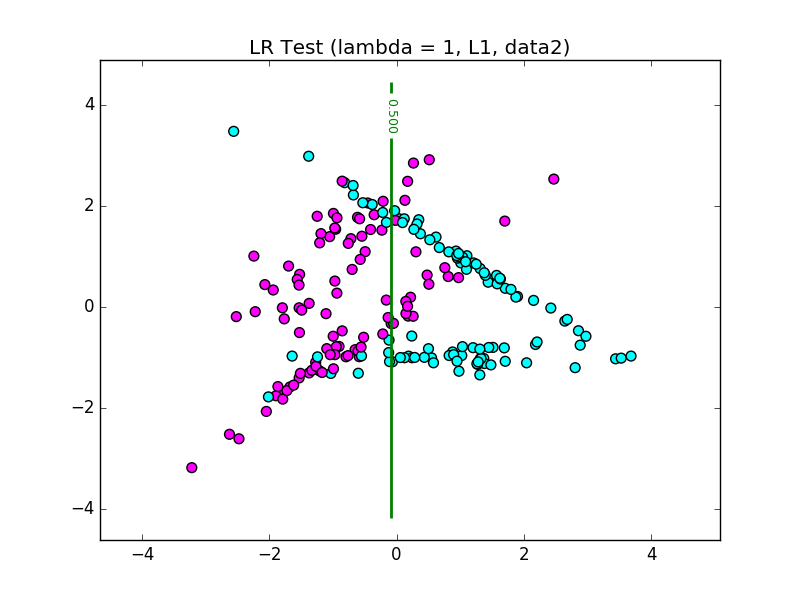
\includegraphics[width=1.2\linewidth]{Part1_data2_test.png}
  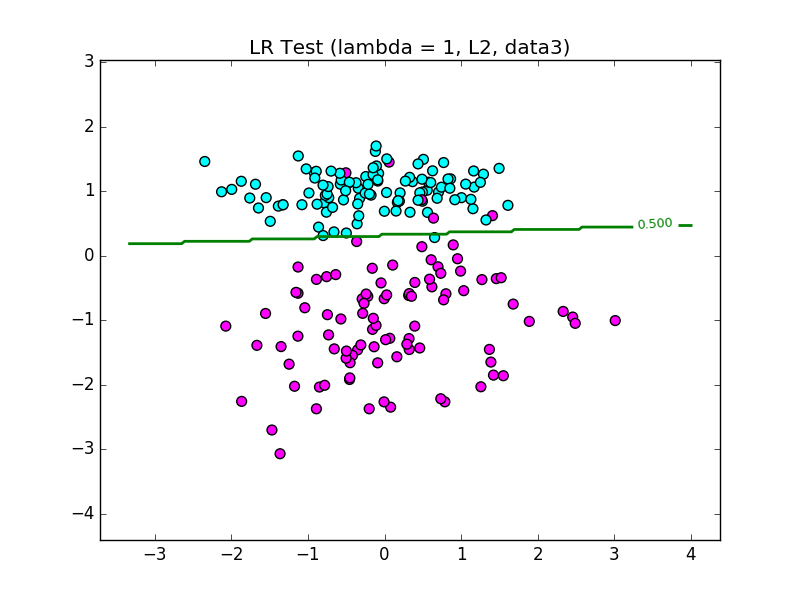
\includegraphics[width=1.2\linewidth]{Part1_data3_test.png}
  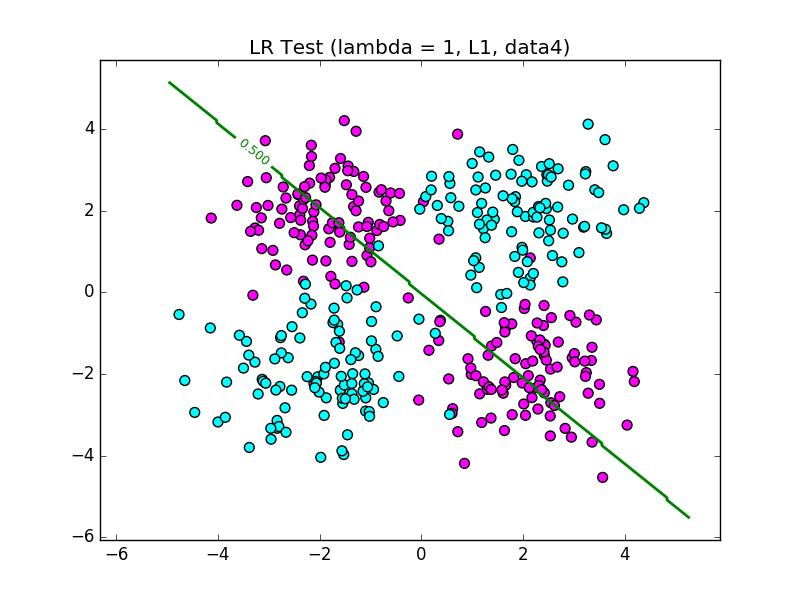
\includegraphics[width=1.2\linewidth]{Part1_data4_test.png}
\end{multicols}
\caption{Decision boundaries for test data}
\end{figure}


\section{Support Vector Machine}
In this section, we explore various versions of the dual form of support vector machines, first with slack variables and then with generalized kernel functions.

\subsection{Dual form with slack variables}
We here implement a dual form of linear SVMs with slack variables. More specifically, we solve the following optimization problem with respect to $\alpha$:
$$\max_\alpha -\frac{1}{2}|\sum_i \alpha_i y^{(i)} x^{(i)}|^2 + \sum_i \alpha_i$$
$$\text{s.t.} \sum_i \alpha_i y^{(i)} = 0$$
$$0 \leq \alpha_i \leq C, 1 \leq i \leq n$$
Written another way, this maximization problem can be framed as a minimization problem:
$$\min_\alpha \frac{1}{2} x^T P x + q^T x$$
$$\text{s.t.} G x \leq h$$
$$ Ax = b $$
where $b=0$ and
$$x=
\begin{bmatrix}
  \alpha_0 \\
  \alpha_1 \\
  \vdots      \\
  \alpha_n \\
\end{bmatrix},
q=
\begin{bmatrix}
  -1 \\
  -1 \\
  \vdots \\
  -1 \\
\end{bmatrix},
A^T=
\begin{bmatrix}
  y_0 \\
  y_1 \\
  \vdots \\
  y_{n-1} \\
\end{bmatrix},
G=
\begin{bmatrix}
  I \\
  -I \\
\end{bmatrix},
$$
where $I$ and $-I$ are the identity and negative identity matrix respectively. Furthermore,
$$
P=
\begin{bmatrix}
  x_0^2 y_0^2             & x_0 y_0 x_1 y_1         & \dots  & x_0 y_0 x_{n-1} y_{n-1}\\
  x_1 y_1 x_0 y_0         & x_1^2 y_1^2             & \dots  & x_1 y_1 x_{n-1} y_{n-1}\\
  \vdots                  & \vdots                  & \ddots & \vdots \\
  x_{n-1} y_{n-1} x_0 y_0 & x_{n-1} y_{n-1} x_1 y_1 & \dots  & x_{n-1}^2 y_{n-1}^2\\
\end{bmatrix}
$$
$$
h^T=
\begin{bmatrix}
  C & \dots & C & 0 & \dots & 0 \\
\end{bmatrix}
$$
In the context of the four-point 2D problem, we seek to solve the following optimization:
$$\min_\alpha \frac{1}{2}
\begin{bmatrix}
  \alpha_0 \\
  \alpha_1 \\
  \alpha_2 \\
  \alpha_3 \\
\end{bmatrix}^T
\begin{bmatrix}
  16 & 24 & 0 & 24 \\
  24 & 36 & 0 & 36 \\
  0  & 0  & 0 & 0 \\
  24 & 36 & 0 & 36 \\
\end{bmatrix}
\begin{bmatrix}
  \alpha_0 \\
  \alpha_1 \\
  \alpha_2 \\
  \alpha_3 \\
\end{bmatrix}
+
\begin{bmatrix}
  -1 \\
  -1 \\
  -1 \\
  -1 \\
\end{bmatrix}^T
\begin{bmatrix}
  \alpha_0 \\
  \alpha_1 \\
  \alpha_2 \\
  \alpha_3 \\
\end{bmatrix}
$$
$$\text{s.t.}
\begin{bmatrix}
  1 & 0 & 0 & 0 \\
  0 & 1 & 0 & 0 \\
  0 & 0 & 1 & 0 \\
  0 & 0 & 0 & 1 \\
  -1 & 0 & 0 & 0 \\
  0 & -1 & 0 & 0 \\
  0 & 0 & -1 & 0 \\
  0 & 0 & 0 & -1 \\
\end{bmatrix}
\begin{bmatrix}
  \alpha_0 \\
  \alpha_1 \\
  \alpha_2 \\
  \alpha_3 \\
\end{bmatrix}
\leq
\begin{bmatrix}
  C \\
  C \\
  C \\
  C \\
  0 \\
  0 \\
  0 \\
  0 \\
\end{bmatrix},
\begin{bmatrix}
  2 \\
  3 \\
  -1 \\
  -2 \\
\end{bmatrix}
\begin{bmatrix}
  \alpha_0 \\
  \alpha_1 \\
  \alpha_2 \\
  \alpha_3 \\
\end{bmatrix}
= 0 $$

Solving for $x$ when $C=1$, we get that $
\begin{bmatrix}
  \alpha_0 & \alpha_1 & \alpha_2 & \alpha_3
\end{bmatrix}^T
=
\begin{bmatrix}
  0.1875 & 0 & 0.3750 & 0 &
\end{bmatrix}^T
$. This indicates that the first and third samples are support vectors because $0 \leq \alpha_i \leq C$. \\

Our implementation of the dual form of SVMs with slack variables was run on each of the four 2D datasets provided. With $C=1$, the decision boundaries and classification error rates were determined. This information is summarized in Figure 2 and Table 2, respectively. As can be seen from the classification error rates in training and validation, depending on the values of the trained parameters and the spread of the datasets, the classification error could be greater for the training data (as in dataset 2), for the validation data (as in dataset 4), or equal (as in dataset 1). Generally however, the linear separator performed best on linearly separable data and classification accuracy in training, validation, and testing datasets clearly suffered for datasets that were not linearly separable (especially datasets 2 and 4).

It is interesting to note that due to numerical rounding and errors, the $\alpha$ values obtained were not exactly equal to 0 or $C$, but instead usually varied by a small threshold. In our case, we chose a threshold of $0.00001$ in order to filter out $\alpha$ values extremely close to 0 or $C$ and select for "true" support vectors. Varying this threshold however could change the classification of data as support vectors or not, and this could ultimately affect the accuracy and error rate of our classifier.

\begin{figure}[width=\linewidth]
\centering
\begin{multicols}{2}
  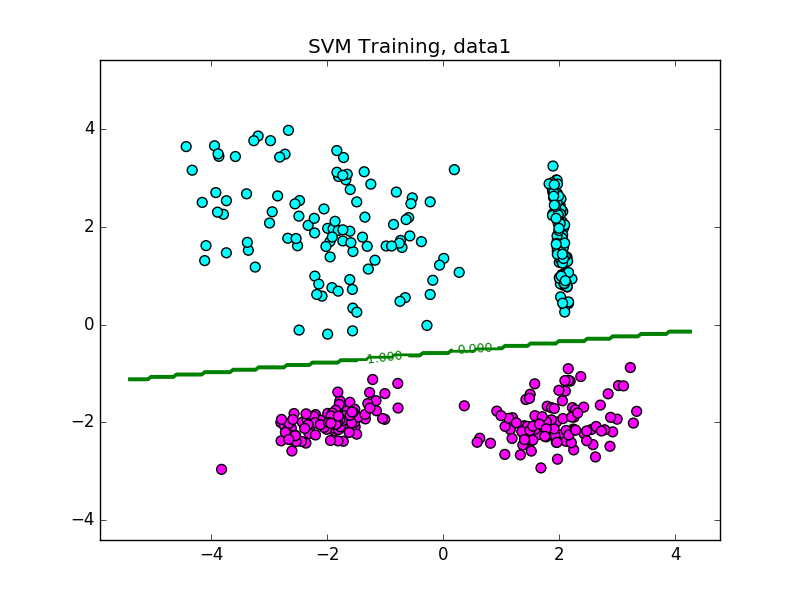
\includegraphics[width=1.2\linewidth]{code/P2/data1,training.png}
  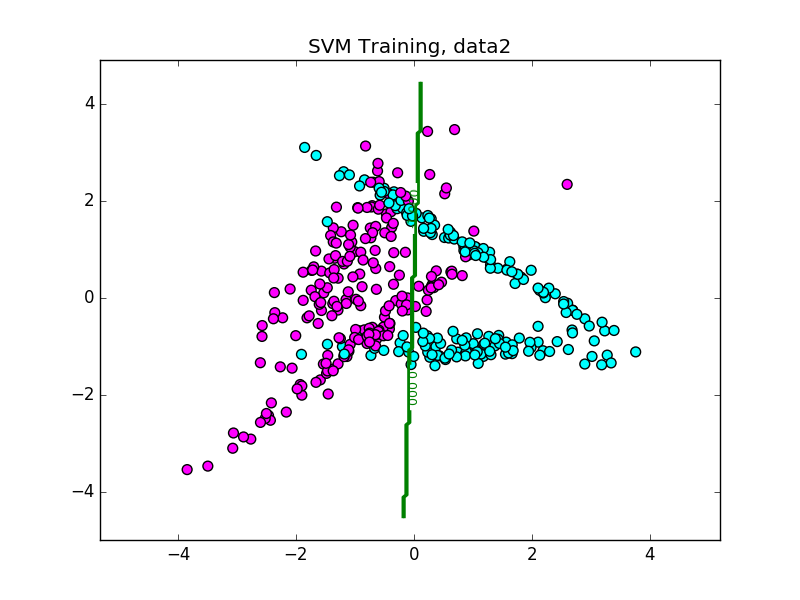
\includegraphics[width=1.2\linewidth]{code/P2/data2,training.png}
  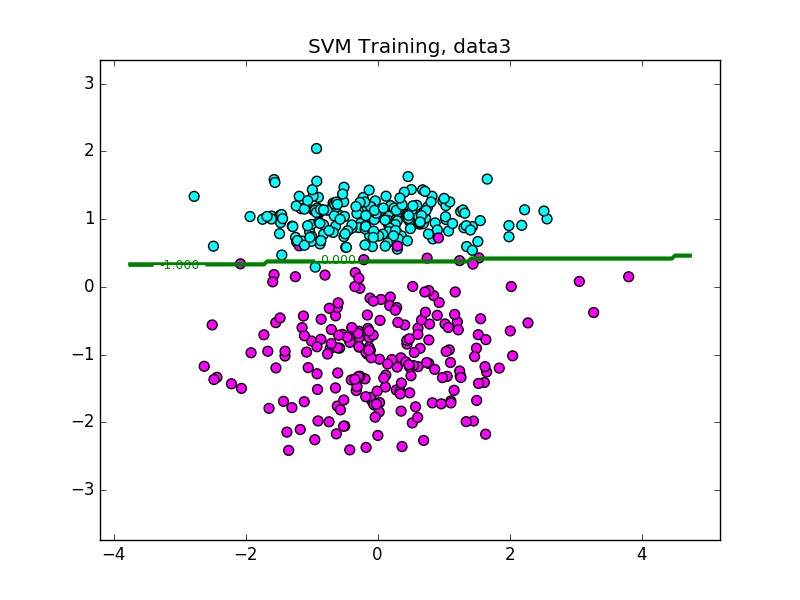
\includegraphics[width=1.2\linewidth]{code/P2/data3,training.png}
  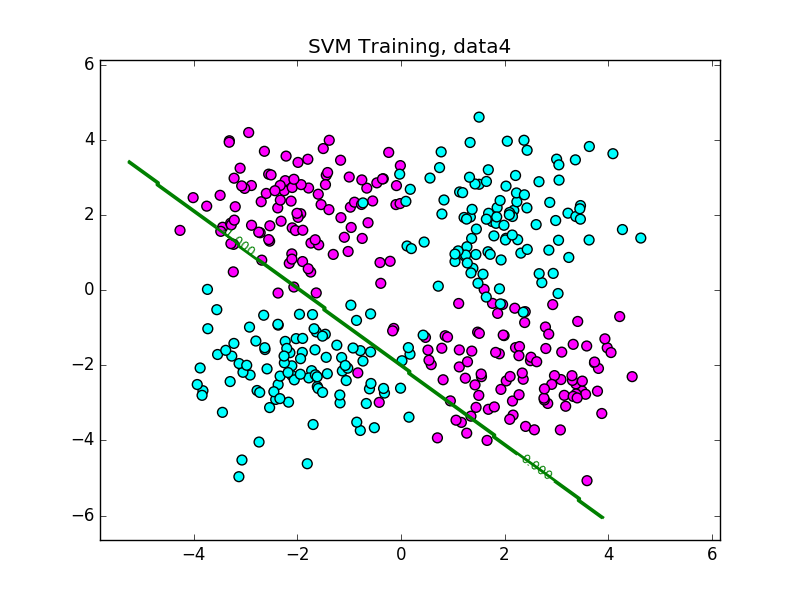
\includegraphics[width=1.2\linewidth]{code/P2/data4,training.png}
  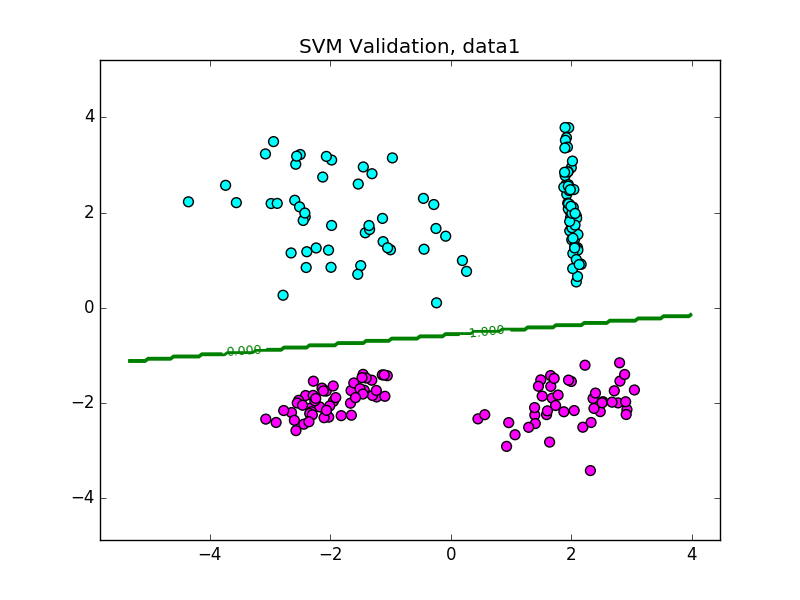
\includegraphics[width=1.2\linewidth]{code/P2/data1,validation.png}
  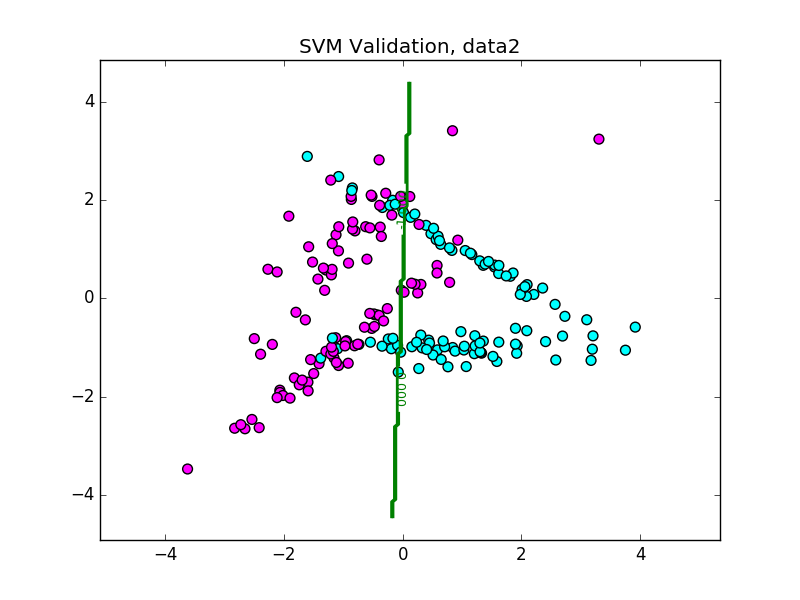
\includegraphics[width=1.2\linewidth]{code/P2/data2,validation.png}
  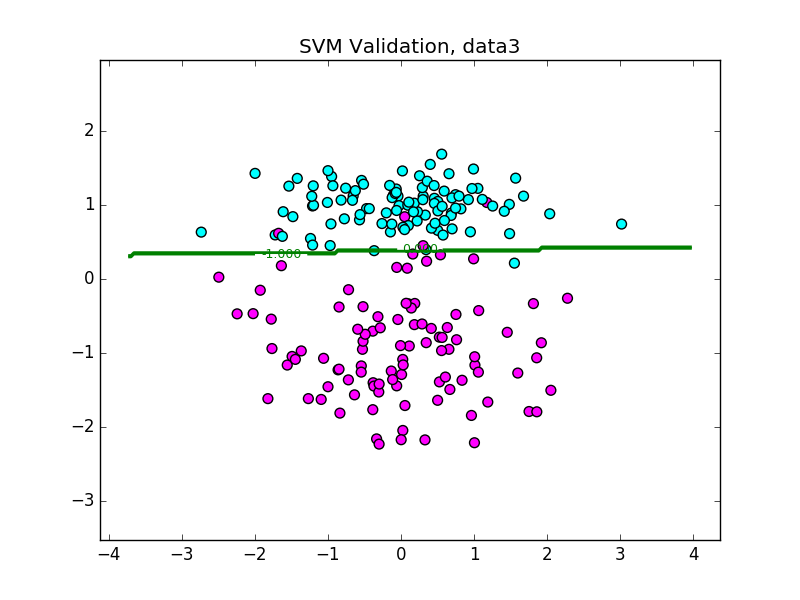
\includegraphics[width=1.2\linewidth]{code/P2/data3,validation.png}
  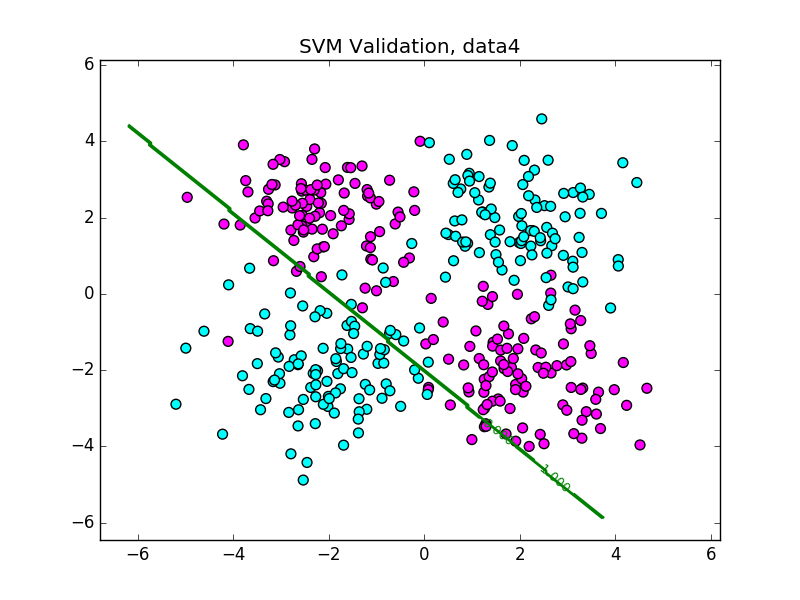
\includegraphics[width=1.2\linewidth]{code/P2/data4,validation.png}
\end{multicols}
\caption{Training and validation decision boundary}
\end{figure}

\begin{table}
  \begin{center}
    \begin{tabular}{ | c | c | c | }
      \hline
      Dataset & Training error rate & Validation error rate \\ \hline
      1       & 0.0                 & 0.0                   \\ \hline
      2       & 0.1775              & 0.09                  \\ \hline
      3       & 0.02                & 0.015                 \\ \hline
      4       & 0.3                 & 0.305                 \\ \hline
    \end{tabular}
  \end{center}
  \caption{Training and validation error rates}
\end{table}

\subsection{Dual form with kernels}
We here extend our dual form SVM to take kernel functions and kernel matrices as input. This has important implications for a number of reasons including performance and minimizing the cost of operations, as well as space and storage. We here implemented the dual form of SVMs with kernels for two kernel functions: (1) linear kernels, and (2) Gaussian radial basis function (RBF) kernels, while varying the value of $C$. Classification for an SVM using the Gaussian RBF kernel with $C$ values of $0.1$ and $100$ is illustrated for each of the four datasets in Figure 3. As can be seen from the plots for $C=0.1$ and $C=100$, as the value of $C$ increases, the model seeks to fit the data more closely. This is because at large values of $C$, which is the regularization parameter, slackness is penalized more. Thus, slack variables which allow the soft-SVM to have some training errors in order to be more generalizable, appear less at extremely large values of $C$ and the model is forced to more closely fit the training data.

\begin{figure}[width=\linewidth]
\centering
\begin{multicols}{2}
  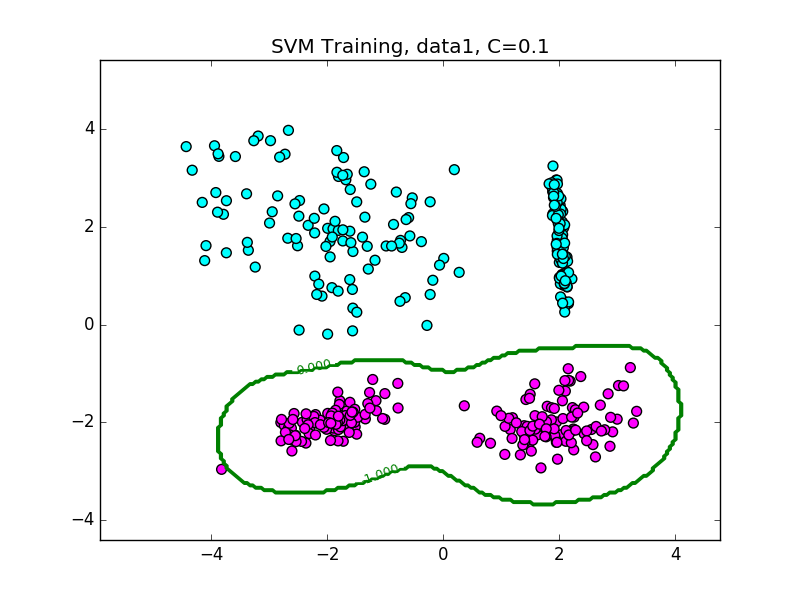
\includegraphics[width=1.2\linewidth]{code/P2/rbf_training,C=01,data1.png}
  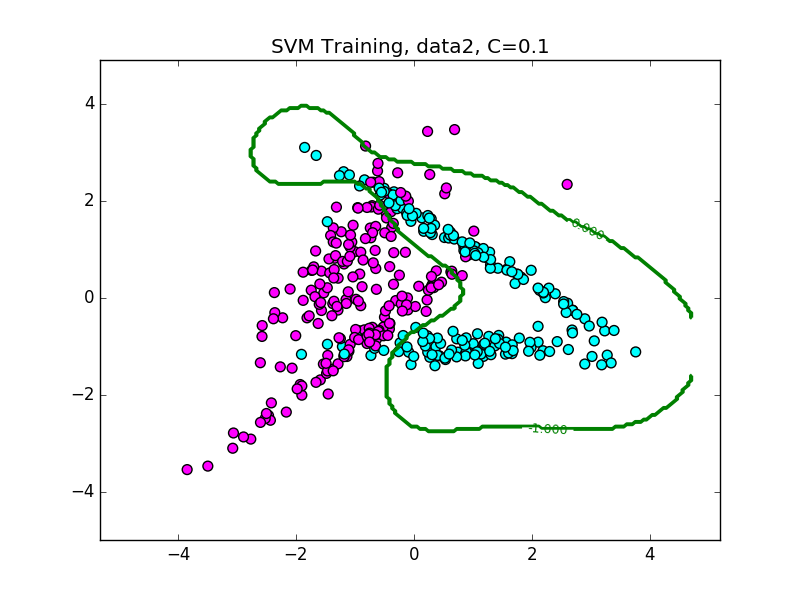
\includegraphics[width=1.2\linewidth]{code/P2/rbf_training,C=01,data2.png}
  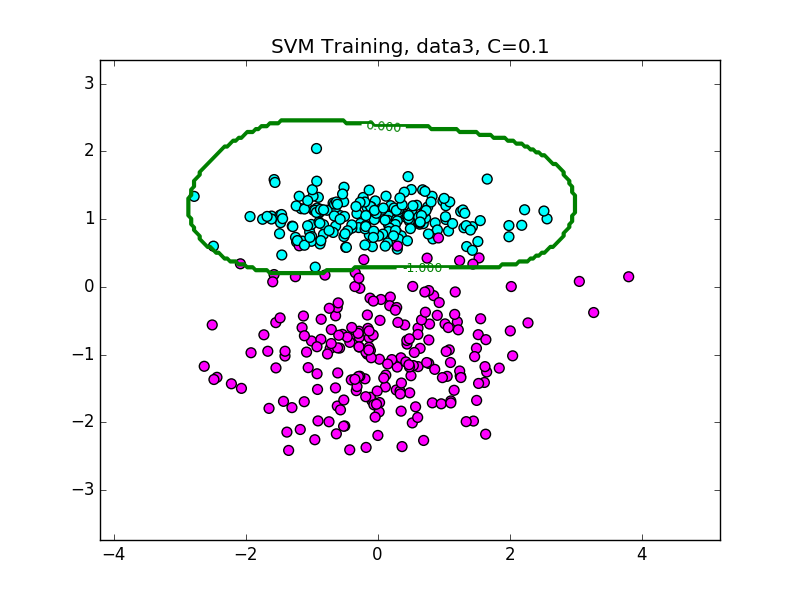
\includegraphics[width=1.2\linewidth]{code/P2/rbf_training,C=01,data3.png}
  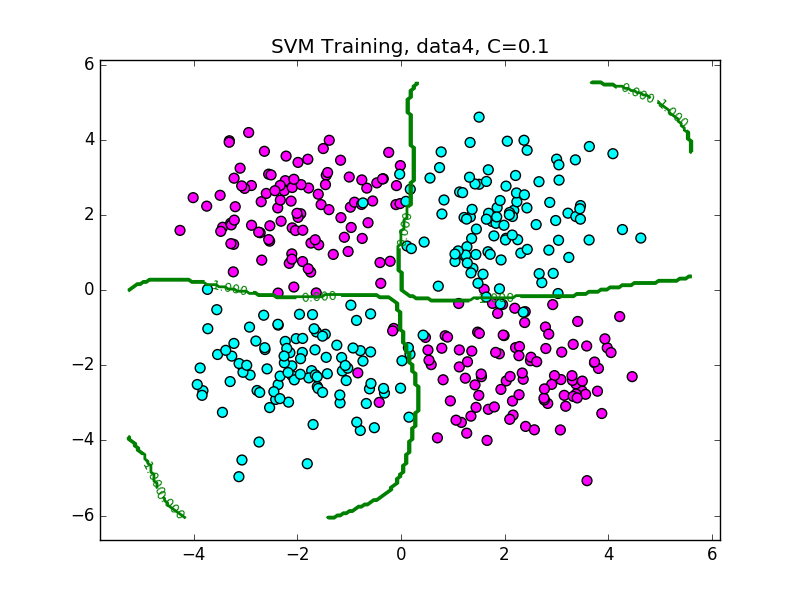
\includegraphics[width=1.2\linewidth]{code/P2/rbf_training,C=01,data4.png}
  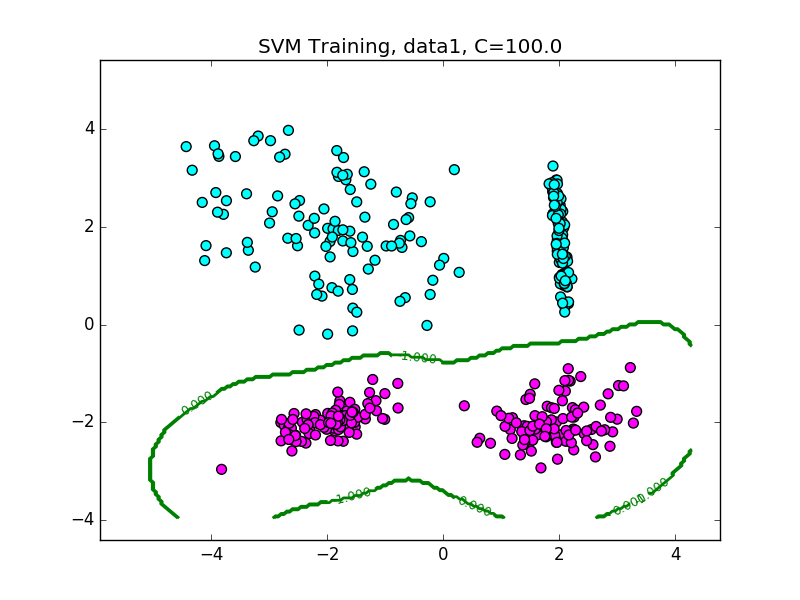
\includegraphics[width=1.2\linewidth]{code/P2/rbf_training,C=100,data1.png}
  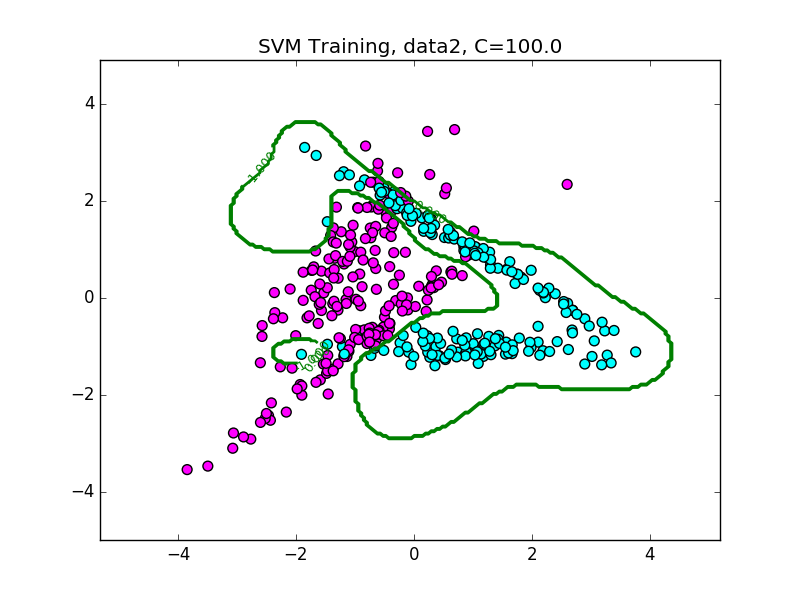
\includegraphics[width=1.2\linewidth]{code/P2/rbf_training,C=100,data2.png}
  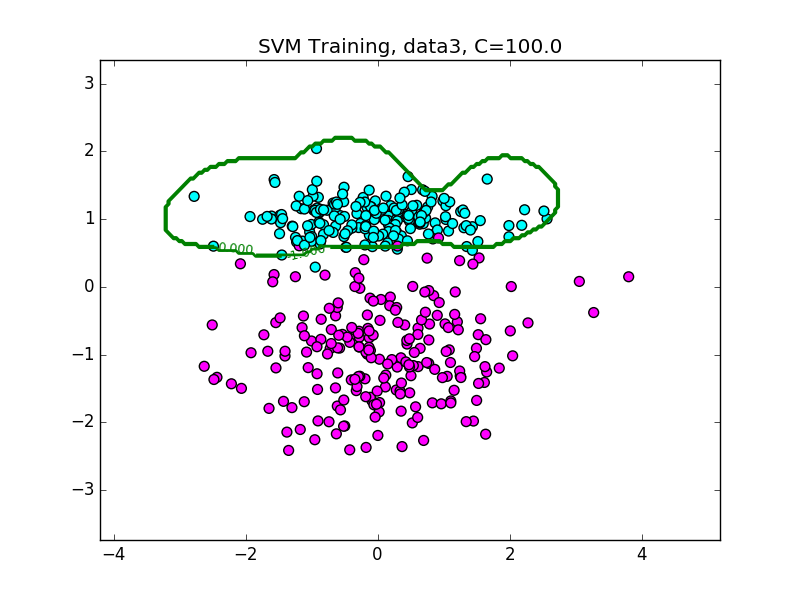
\includegraphics[width=1.2\linewidth]{code/P2/rbf_training,C=100,data3.png}
  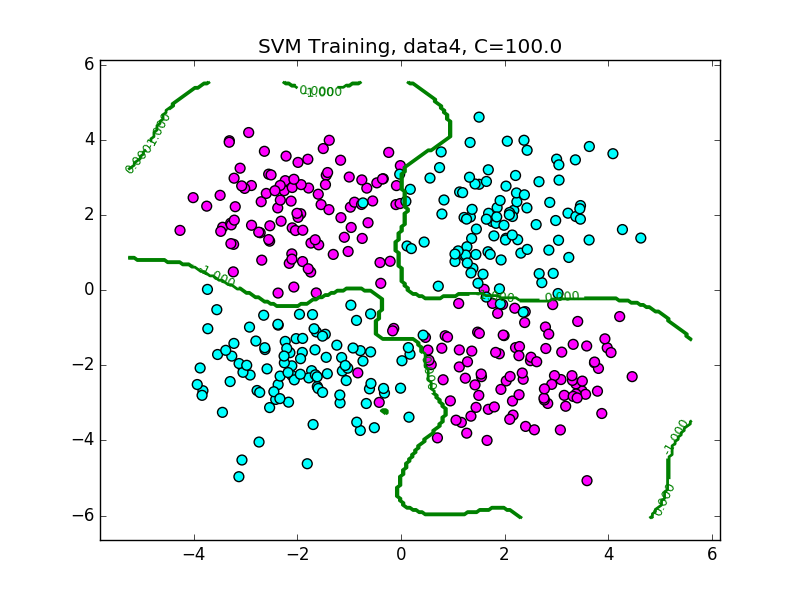
\includegraphics[width=1.2\linewidth]{code/P2/rbf_training,C=100,data4.png}
\end{multicols}
\caption{Training and validation decision boundary}
\end{figure}

Furthermore, as the value of $C$ increases, on a conceptual level, the margin error should decrease. This makes intuitive sense because $C$ is the regularization parameter on the slack variables. Thus, as the penalization on the slack variables increases, the weights must increase in order to accommodate for a closer fit to the training data. The margin error, which is defined as the $\frac{1}{||w||}$ should therefore decrease. This is only true up to a point however, because at extremely high values of $C$ when all slackness has been virtually eliminated, the weights will only continue to increase until it is able to completely fit the data. Beyond this point, increasing the value of $C$ should not force the weights to increase as well if they can sufficiently capture the data, and thus, the margin error should plateau after a certain point.

As the value $C$ was increased, the number of support vectors generally did not show any noticeable or significant trends with a linear kernel. For all the data sets for varying values of $C$, the number of support vectors stayed roughly constant at around 3 or 4. However, for the Gaussian RBF kernel, the number of support vectors generally increased as the value of $C$ increased until a certain point (generally around $C=1$), after which the number of support vectors plateaued or even decreased. This data for the Gaussian RBF is summarized in Table 3.

\begin{table}
  \begin{center}
    \begin{tabular}{ | c | c | c | c | c | c | }
      \hline
              & $C=0.01$ & $C=0.1$ & $C=1$ & $C=10$ & $C=100$ \\ \hline
      1       & 0        & 29      & 45    & 49     & 48      \\ \hline
      2       & 0        & 21      & 32    & 32     & 36      \\ \hline
      3       & 2        & 16      & 28    & 25     & 20      \\ \hline
      4       & 0        & 35      & 79    & 78     & 75      \\ \hline
    \end{tabular}
  \end{center}
  \caption{Number of support vectors by C value}
\end{table}

It is interesting to note that simply maximizing the geometric margin $\frac{1}{||w||}$ on the training set is not an optimal criterion for selecting $C$. This is because this decrease in the value of $C$ would maximize the geometric margin, but would additionally reduce the number of support vectors. Furthermore, at extremely small values of $C$, the penalization on the slackness variables drops out, and the slack variables are able to grow without bound. In this case, the weights would go to 0, and the slack variables would adjust to fully account for the data. This would not sufficiently train the weights of the model, and would instead overfit the slack variables to the training set but result in extremely poor classification accuracy for other data sets. An alternative criterion which could be used for selecting $C$ could be to optimize the ratio of the number of support vectors to the total number of samples in the training data. This would ensure that the model trained would fully represent the data without extreme overfitting or underfitting.

\section{Pegasos}

In this section, we use the Pegasos algorithm to solve the following formulation of Soft-SVM:
$$\min \frac{\lambda}{2} ||w||^2 + \frac{1}{n} \sum_{i=1}^{N}  \max \{0,1 - y_i(w^T x_i)\}$$
We choose to use Pegasos because it combines together multiple good ideas such as hinge loss, L2 regularization, stochastic (sub)-gradient descent, and a decaying step-size. Table 4 shows the impact of $\lambda$ (regularization constant) on the margin. It indeed matches our understanding of the objective function because lower regularization means larger slack variables which lead to smaller margins. The reason for this is because $1-\epsilon_i$ governs the width of the margin.

\begin{table}
  \begin{center}
    \begin{tabular}{ | c | c | c | c | c | c | c | c | c |}
      \hline
       $\lambda$& $2^1$       & $2^{-1}$&  $2^{-3}$& $2^{-5}$&  $2^{-7}$&  $2^{-10}$ \\ \hline
       margin       & $\infty$     & $1.134$&   $0.820$& $0.642$&  $0.547$&   $0.389$  \\ \hline

    \end{tabular}
  \end{center}
  \caption{SVM margin as a function of $\lambda$}
\end{table}

After creating the regular Pegasos algorithm, we then proceeded to create the kernelized version of the algorithm to solve the following Soft-SVM problem:
$$\min \frac{\lambda}{2} ||w||^2 + \frac{1}{n} \sum_{i=1}^{N}  \max \{0,1 - y_i(w^T \phi(x_i))\}$$

This formulation outputs an array of $\alpha$ values that enables us to make predictions through utilizing the following equation:
$$F(x) = \sum_{j=1}^{l} \alpha_jK(x_j,x)$$
(Note that due to the fact that the $\alpha$ values are able to be negative we don't multiply by $y$). Additionally, we did find that this kernelized algorithm gave us a sparse solution similar to what we saw with the dual SVM. Using $\lambda = 0.02$ and $\gamma = 2^2$ we only saw 57 nonzero $\alpha$ values out of a possible 400. Using a fixed $\lambda$ value of $0.02$, table 5 shows the relationship between $\gamma$ and the number of support vectors produced.

\begin{table}
  \begin{center}
    \begin{tabular}{ | c | c | c | c | c | c | c |}
      \hline
       $\gamma$   & $2^2$       & $2^{1}$&  $2^{-1}$& $2^{-2}$\\ \hline
       \# of SVMs & $57$     & $37     $&  $30$     & $28$ \\ \hline

    \end{tabular}
  \end{center}
  \caption{Number of SVMs as a function of $\gamma$}
\end{table}
Furthermore we saw that the margins of our decision boundaries increased as $\gamma$ decreased. This makes intuitive sense $\gamma$ is negatively correlated to bandwidth. Our results compared very well against the results we obtained in the previous section. We saw that the exact performance depended heavily on what we set as our max epochs. Ultimately, this leads to a tradeoff between run time and classification accuracy.

\section{Handwritten digit recognition}
Here we investigate the performance of the algorithms implemented on handwritten digit recognition in the MNIST dataset.

\subsection{Logistic regression versus linear SVM}

The logistic regression algorithm with L1 regularization from problem 1 is compared with the linear SVM classifier from problem 2. The testing error rates, following optimization of hyperparameters through validation on the validation datasets, are summarized in Table 5 for both logistic and linear SVM classifiers. For the linear SVM, optimal values for $C \in [0.2, 0.4, 0.6, 0.8, 1]$ are indicated in parentheses.

\begin{table}
  \begin{center}
    \begin{tabular}{ | c | c | c | }
      \hline
                     & Logistic (L1)    & Linear SVM       \\ \hline
      1 vs. 7        & 0.017            & 0.013 (0.2)      \\ \hline
      3 vs. 5        & 0.057            & 0.053 (0.2)      \\ \hline
      4 vs. 9        & 0.057            & 0.057 (0.2)      \\ \hline
      even vs. odd   & 0.115            & 0.113 (0.2)      \\ \hline
    \end{tabular}
  \end{center}
  \caption{Error rates for un/normalized data}
\end{table}

Overall, the linear SVM performed slightly better than the logistic regression under L1 regularization. Similar results were found for logistic regression under L2 regularization. It makes intuitive sense that the even vs. odd classification task performed with the worst accuracy rate of all of the classification tasks presented. This is because even vs. odd numbers do not necessarily have distinctive physical features belonging to the overall class, so training the model was likely extremely general with low specificity regarding each individual number.

This analysis was conducted for both normalized data and not normalized data. Interestingly, whether or not the data was normalized did not affect the training or testing error rates. Furthermore, examining some of the misclassified images reveals that this classification does in fact make sense in the overall scope of the algorithms used, where in some cases it was even difficult to classify by the images by human examination. Some of the training errors in the 1 versus 7 classification are illustrated in Figure 4.

\begin{figure}[width=\linewidth]
\centering
\begin{multicols}{2}
  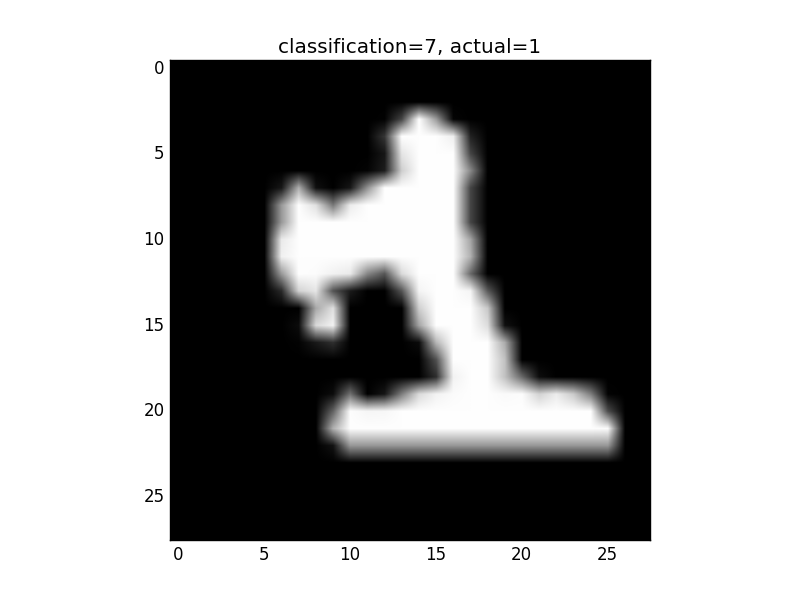
\includegraphics[width=1.2\linewidth]{code/P4/error,1.png}
  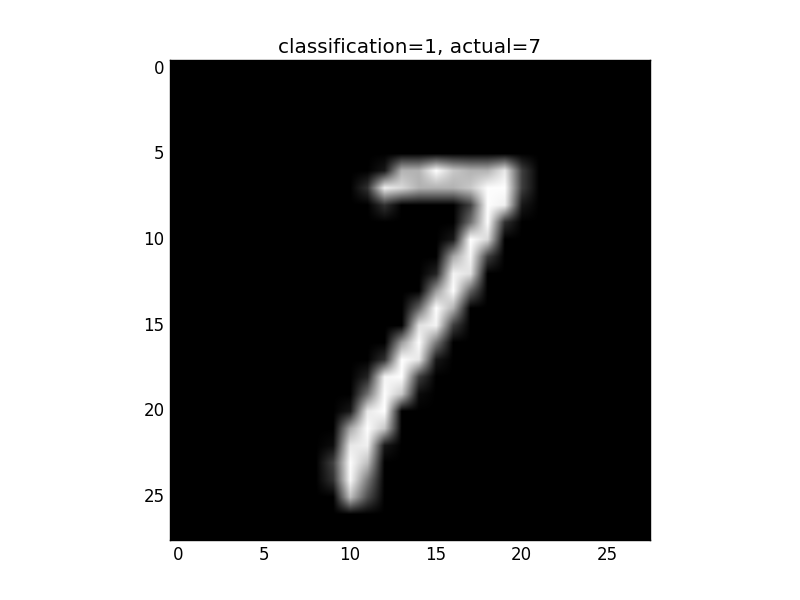
\includegraphics[width=1.2\linewidth]{code/P4/error,7.png}
\end{multicols}
\caption{Classification errors in test set}
\end{figure}

\subsection{Gaussian RBF SVM}

We additionally investigated the classification accuracy of the Gaussian RBF SVM on the MNIST dataset with selection of hyperparameters through validation. Here, $C$ was selected from possible $C$ values of $[0.2, 0.4, 0.6, 0.8, 1]$ and $\gamma$ was selected from possible values of $[0.5, 1, 5, 10]$. For each of the pairwise classification tasks presented previously when evaluating the MNIST data using logistic regression and a linear SVM, optimal values for $C$ and $\gamma$ for the Gaussian RBF SVM were selected. These sets of hyperparameters were each associated with a classification error rate in the testing dataset. These results are presented in Table 6.

\begin{table}
  \begin{center}
    \begin{tabular}{ | c | c | c | c | }
      \hline
                     & $C^*$          & $\gamma^*$           & Testing error      \\ \hline
      1 vs. 7        & 0.4            & 0.5                  & 0.0                \\ \hline
      3 vs. 5        & 0.4            & 0.5                  & 0.0                \\ \hline
      4 vs. 9        & 0.4            & 0.5                  & 0.0                \\ \hline
      even vs. odd   & 0.4            & 0.5                  & 0.0                \\ \hline
    \end{tabular}
  \end{center}
  \caption{Classification using Gaussian RBF SVM}
\end{table}

As seen previously with logistic regression and the linear SVM, normalization of the data did not affect the optimal values of $C$ or $\gamma$, or the classification testing accuracy with a Gaussian RBF SVM. Overall however, the Gaussian RBF SVM generally performed better than both the logistic regression (with L1 or L2 regularization) and the linear SVM. It is worth noting however, that the Gaussian RBF SVM ran much slower than the logistic and linear SVM implementations. There is a tradeoff to be noted here therefore between runtime and testing accuracy, as is commonly seen in many algorithms and systems. Thus, although the Gaussian RBF SVM dramatically improved on the linear classifiers in terms of accuracy, it also suffered dramatically in terms of runtime and performance.

\subsection{Pegasos}

Comparing the linear and Gaussian SVMs with Pegasos, we can evaluate all algorithms based on classification accuracy as well as performance. Pegasos generally ran with slightly improved accuracies over the linear SVM and logistic regression, with error rates of $0.007, 0.057,$ and $0.043$ for 1 vs. 7, 3 vs. 5, and 4 vs. 9, respectively. The accuracies across most of the algorithms were therefore extremely comparable, with the exception of the Gaussian kernel SVM which ran with 0\% testing error.

The performance in terms of runtime was additionally investigated for each of these algorithsm. These runtimes, presented in seconds, is summarized in Table 7. Note that here, we have chosen the 4 vs. 9 classification task to examine in more detail, but the results from this dataset should generalize well to other classification tasks including 1 vs. 7, 3 vs. 5, and even vs. odd.

\begin{table}
  \begin{center}
    \begin{tabular}{ | c | c | c | c | c | }
      \hline
             & Logistic     & Linear   & Gaussian SVM & Pegasos    \\ \hline
      200    & 0.5          & 40           & 200           & 6          \\ \hline
      300    & 0.8          & 87           & 348           & 8          \\ \hline
      400    & 0.5          & 161          & 620           & 12         \\ \hline
      500    & 0.9          & 217          & 891           & 16         \\ \hline
    \end{tabular}
  \end{center}
  \caption{Runtimes of classification algorithms}
\end{table}

The above numbers for Pegasos are under the parameters where $\lambda = 2^{-10}$ and $max\_epochs = 100$. The runtime of Pegasos is dependent upon the values for these parameters however, and increasing the maximum number of epochs would accordingly increase the runtime of the algorithm. This follows directly from the implementation of the algorithm, in which a greater number of epochs results in more iterations of the for loop, thereby increasing the runtime of the algorithm. Similarly, as the value of $\lambda$ increased, the runtime of the overall algorithm increased. This is because the step size is inversely proportional with the value of $\lambda$. Thus, at small values of $\lambda$, the step size is larger, and we thus approach the margin more quickly. If this is the case, then fewer computation steps are required and thus, a faster runtime is associated with a smaller value of $\lambda$.

Overall, it seems that logistic regression and Pegasos present the ideal balance in the tradeoff between runtime and classification accuracy. While the Gaussian SVM had a perfect classification accuracy, the algorithm required more than 30 times longer to run to completion compared with Pegasos, with this factor increasing as the number of training samples increased. On the other side of the spectrum, the logistic regression ran fastest out of all the algorithms, although it had slightly worse accuracy compared with Pegasos and the Gaussian SVM. Thus, depending on the needs of the system, both logistic regression and Pegasos present algorithms which maintain acceptable classification accuracy while remaining scalable to large datasets with many features.

\end{document}


% This document was modified from the file originally made available by
% Pat Langley and Andrea Danyluk for ICML-2K. This version was
% created by Lise Getoor and Tobias Scheffer, it was slightly modified
% from the 2010 version by Thorsten Joachims & Johannes Fuernkranz,
% slightly modified from the 2009 version by Kiri Wagstaff and
% Sam Roweis's 2008 version, which is slightly modified from
% Prasad Tadepalli's 2007 version which is a lightly
% changed version of the previous year's version by Andrew Moore,
% which was in turn edited from those of Kristian Kersting and
% Codrina Lauth. Alex Smola contributed to the algorithmic style files.
